\section{Numerical Methods for Elliptic PDEs}
\label{sec:numerical-methods-for-elliptic-pdes}

\subsection{Finite Difference}

\begin{figure}
    \centering
    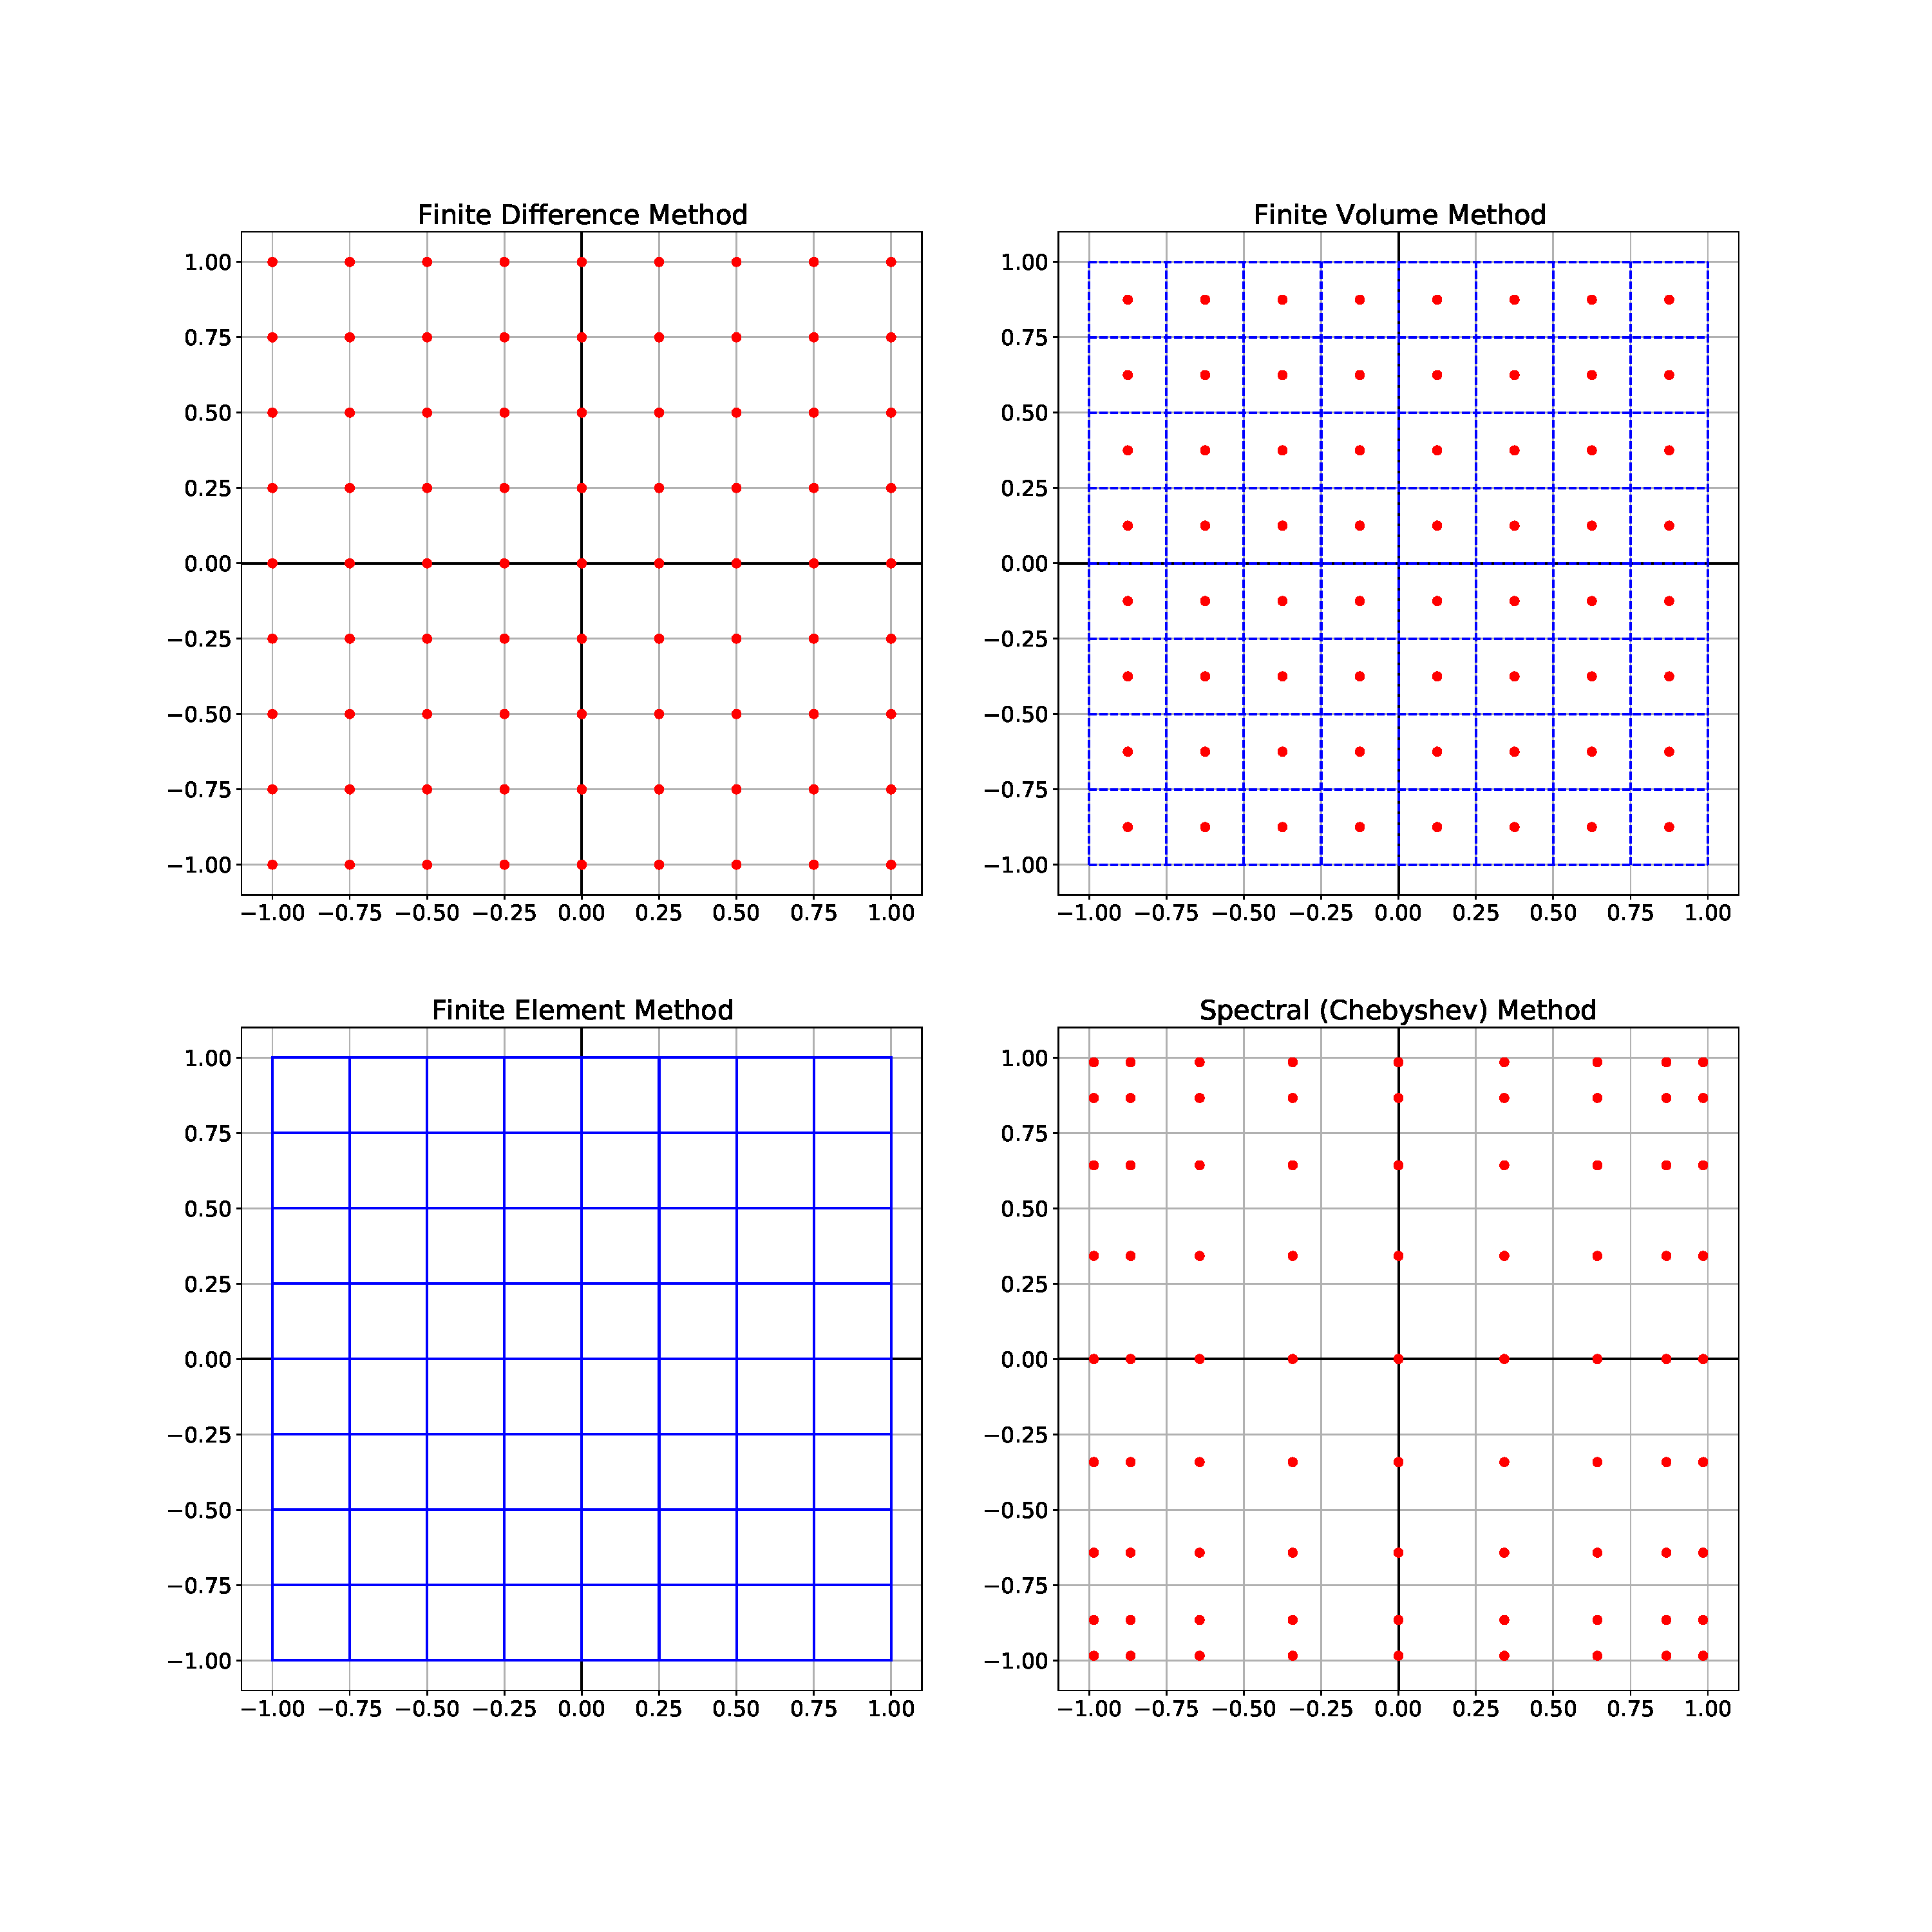
\includegraphics[width=0.8\columnwidth]{figures/PDE_discretization_methods.pdf}
    \caption{Discretization Methods. Top Left: Finite difference grid based on a mesh of points or nodes. Top Right: Finite volume mesh made of cells (dashed blue boxes) with cell averages in the center (red points). Bottom Left: Finite element mesh where each blue box is an element with a shape function defined at all points within the element. Bottom Right: Spectral mesh made up of a tensor of Chebyshev nodes.}
    \label{fig:discretization_methods}
\end{figure}

If $\Omega$ is on a logically rectangular domain (i.e. 2D Cartesian plane), perhaps the simplest discretization of the domain $\Omega$ is by collocating a mesh of points throughout the domain. Given upper and lower bounds in both directions, $[x_l, x_u], [y_l, y_u]$, the x- and y-location of each point can be defined as
\begin{align}
    x_i &= x_l + i \Delta x,\ \ \ i = 0, 1, ..., N_x-1 \\
    y_i &= y_l + j \Delta y,\ \ \ j = 0, 1, ..., N_y-1
\end{align}
where $N_x, N_y$ is the number of points in the x- and y-direction and grid spacing is defined as
\begin{align}
    \Delta x &= \frac{x_u - x_l}{N_x - 1} \\
    \Delta y &= \frac{y_u - y_l}{N_y - 1}.
\end{align}
These points are shown in the first plot of Figure \ref{fig:discretization_methods}. This type of discretization is known as the {\em finite difference method}. \damyn{(Cite something here?)}. In the finite difference approach, the expressions for the derivatives in a PDE are replaced with Taylor series approximations. For example, a second order accurate, central-difference approximation to the second derivative can be given as
\begin{align}
    \frac{\partial^2 u}{\partial x^2} &= \frac{u(x - \Delta x, y) - 2u(x, y) + u(x + \Delta x, y)}{\Delta x^2} + \mathcal{O}(\Delta x^2)
\end{align}
and if we let $u(x_i, y_j) = u_{i,j}$, then we can write this as
\begin{align}
    \frac{\partial^2 u}{\partial x^2} &= \frac{u_{i-1,j} - 2u_{i,j} + u_{i+1,j}}{\Delta x^2} + \mathcal{O}(\Delta x^2).
\end{align}
Using these Taylor Series expansions, we can replace the continuous Poisson's equation \ref{eq:variable_poisson} with the discrete system of equations:
\begin{align}
    \frac{u_{i-1,j} - 2u_{i,j} + u_{i+1,j}}{\Delta x^2} + \frac{u_{i,j-1} - 2u_{i,j} + u_{i,j+1}}{\Delta y^2} &= f_{i,j}.
    \label{eq:poisson_FD}
\end{align}
For each grid point $i = 0, ..., N_x - 1$, $j = 0, ..., N_y - 1$ this expression forms a linear system with $(N_x-1) \times (N_y-1)$ unknowns.

The system that is formed from this discretization is sparse and banded. For example, let $N_x = N_y = N$ for simplicity (thus $\Delta x = \Delta y = h$). Index the vector $\textbf{u}$ first by rows, then by columns, such that
\begin{align}
    \textbf{u} = [u_{0,0}, ..., u_{N - 1, 0}, u_{0, 1}, ..., u_{N - 1, 1}, ..., u_{0, N - 1}, ..., u_{N - 1, N - 1}]^T.
\end{align}
The corresponding linear system from \ref{eq:poisson_FD} is the following:
\begin{align}
    \textbf{A} &= \frac{1}{h^2}
    \begin{bmatrix}
        \textbf{D} & \textbf{I}_{N} & \textbf{0} & ... & \textbf{0} \\
        \textbf{I}_{N} & \textbf{D} & \textbf{I}_{N} & ... & \textbf{0} \\
        \textbf{0} & \textbf{I}_{N} & \textbf{D} & ... & \textbf{0} \\
        \vdots & \vdots & \vdots & \ddots & \vdots \\
        \textbf{0} & \textbf{0} & \textbf{0} & ... & \textbf{D}
    \end{bmatrix}
\end{align}
where
\begin{align}
    \textbf{D} &= 
    \begin{bmatrix}
        -4 & 1 & 0 & ... & 0 \\
        1 & -4 & 1 & ... & 0 \\
        0 & 1 & -4 & ... & 0 \\
        \vdots & \vdots & \vdots & \ddots & \vdots \\
        0 & 0 & 0 & ... & -4
    \end{bmatrix}.
\end{align}
We also index the RHS similarly to $u(x,y)$ resulting in a RHS vector $\textbf{f}$. This leads to the linear system
\begin{align}
    \textbf{A} \textbf{u} = \textbf{f} + \textbf{b}
\end{align}
where $\textbf{b}$ contains any updates necessary for any type of boundary condition.

\subsection{Finite Volume}

In a finite volume scheme, the domain is broken up into cells, which can be structured or unstructured polygons (2D) or polyhedrons (3D). The function to approximate is solved for in terms of a cell average. Finite volume schemes are often used to solve equations modeling conservation laws, where the cell quantity is conserved in time through balancing fluxes (what comes in and out of the cell boundaries) and the cell source (what the cell is generating or destroying). In a finite volume scheme, the cell average is updated according to the integral formulation of the conservation law as
\begin{align}
    \frac{\partial}{\partial t} \int_{\Omega_i} \textbf{q} d\Omega_i + \int_{\Gamma_i} \textbf{F}(\textbf{q}) \cdot \hat{n}_i d\Gamma_i + \int_{\Omega_i} \textbf{s} d\Omega_i = 0,
\end{align}
where $\Omega_i$ and $\Gamma_i$ are the cell domains and boundaries, respectively, $\textbf{q}$ is a vector of quantities in each cell, $\textbf{F}$ is a flux function, and $\textbf{s}$ is the cell's source term. In the second plot of Figure \ref{fig:discretization_methods}, the blue dashed lines are the cell boundaries, and the red points are the cell centers. For up to second order schemes, the cell average is collocated at the center of the cell; this changes for higher order schemes.

\subsection{Finite Element}

In a finite element scheme, the domain is broken into elements. These elements can also be structured or unstructured polygons (2D) or polyhedrons (3D), similar to the finite volume method. The PDE to solve is converted into a weak form by multiplying the PDE by a test function $v(x,y)$ and integrating over the domain:
\begin{align}
    \int_{\Omega} v \nabla^2 u d\Omega &= \int_{\Omega} vf d\Omega.
\end{align}
Green's Theorem (i.e., integration by parts) is used to break the LHS into integrals on the domain $\Omega$ and the boundary $\partial \Omega = \Gamma$:
\begin{align}
    -\int_{\Omega} \nabla v \cdot \nabla u d\Omega + \int_{\Gamma} v \frac{\partial u}{\partial n} d\Gamma &= \int_{\Omega} vf d\Omega
    \label{eq:poisson_weak_form}
\end{align}
The idea behind the finite element method is to use basis functions
\begin{align}
    u(x,y) \approx \bar{u} = \sum_{k=1}^{N_k} c_k \phi(x,y)
\end{align}
inside each element $\Omega_i$, where $\Omega = \cup_{i = 1}^{N_{\text{elem}}} \Omega_i$. When the same basis functions for the test functions $v$ are also used, this leads to the Galerkin finite element method. Upon substitution of the above into \ref{eq:poisson_weak_form}, and integrating the basis function with either quadrature or with analytical expressions, a linear system is formed for the coefficients $c_k$.

There are several variations of the finite element method. The method explained above forms a global linear system involving all elements. To avoid this, mapping a physical element to some reference element, makes the contributions from a single element only influence itself and its neighbors. This makes the coefficient matrix in the linear system much more sparse and structured, making it easier to solve. Additionally, by not imposing continuity across element boundaries, one arrives at the discontinuous Galerkin method, where the discontinuities are handled through element fluxes. By choosing certain shape or basis functions, one can derive different variations of the finite element method, including the B-spline finite element method \cite{kagan1998new} and the spectral element method \cite{patera1984spectral}.

\subsection{Spectral Methods}

In spectral methods, the approach is to approximate the solution $u$ as a linear combination of a finite set of orthogonal basis functions
\begin{align}
    u(x,y) = \sum_{i=1}^{N_x} \sum_{j=1}^{N_y} c_{i,j} \phi_{i}(x) \phi_{j}(y)
\end{align}
where the coefficients are chosen to minimize a norm, such as the $L^2$ norm of the residual $r(x,y) = \nabla^2 u(x,y) - f(x,y)$. On a discrete domain, this is similar to requiring $\nabla^2 u(x_i, y_j) = f(x_i, y_j)$ at all interior grid points. As this acts like an interpolation scheme, increasing the number of discretization points on with a fixed interval actually leads to highly oscillatory results. Thus, in spectral methods, it is common to use grid points that are clustered near the ends of the interval, such as Chebyshev points, defined on an interval $[a,b]$ as
\begin{align}
    x_i &= a + \frac{1}{2}(b - a)\Big(1 + \cos \big( \pi (1 - \frac{i}{N + 1}) \big) \Big), i = 0, ..., N + 1.
\end{align}
These points are shown on the last plot of Figure \ref{fig:discretization_methods}. With a good basis of grid points, spectral methods can achieve very fast convergence. The linear system formed by this method will be dense as it functions like a high-order interpolation scheme. However, as convergence is much faster than high-order finite difference methods, one can use far fewer points on a grid, so the size of the system is kept small. If one uses Fourier series as the basis functions $\phi$, one can accelerate the solution of the linear system using fast Fourier Transform algorithms. Though, due to the periodic nature of the Fourier series, it is more difficult to implement non-periodic boundary conditions (\cite{leveque2007finite}, \cite{townsend2015automatic}).

% [TODO: Rework this section]
%
% In each of the methods presented above, the function approximation is found by forming and solving a linear system. In spectral methods, one uses integral transformations such as the Fourier or Laplace Transforms to differentiate. For example, the Fourier Transform of a function is given as
% \begin{align}
%     F(k) = \mathcal{F}[f(x)] = \frac{1}{\sqrt{2\pi}} \int_{-\infty}^{\infty} f(x) e^{ikx} dx
% \end{align}
% with it's inverse
% \begin{align}
%     f(x) = \mathcal{F}^{-1}[F(k)] = \frac{1}{\sqrt{2\pi}} \int_{-\infty}^{\infty} F(k) e^{ikx} dk.
% \end{align}
% The strength of these methods show when considering the derivatives of $f(x)$:
% \begin{align}
%     \frac{\partial^n f}{\partial x^n} &= \frac{\partial^n}{\partial x^n} \frac{1}{\sqrt{2\pi}} \int_{-\infty}^{\infty} F(k) e^{ikx} dk \\
%     &= \frac{1}{\sqrt{2\pi}} \int_{-\infty}^{\infty} (ik)^{n} F(k) e^{ikx} dk
% \end{align}
% So any $nth$ derivative can be expressed in terms of a Fourier and inverse Fourier transform:
% \begin{align}
%     \frac{\partial^n f}{\partial x^n} &= \mathcal{F}^{-1}[(ik)^n \mathcal{F}[f(x)]].
% \end{align}
% In practice, one can use fast algorithms such as the famous Fast Fourier Transform to perform this arithmetic.
%
% A minor drawback to this method is the need to work on a periodic domain in order for the Fourier Transform to function properly. This makes enforcing boundary conditions difficult. Thus, extensions to spectral methods include using a better basis of points than evenly spaced points, such as Chebyshev nodes. Chebyshev nodes defined in the interval $(-1, 1)$ are given as
% \begin{align}
%     x_k = \cos \Big( \frac{2k - 1}{2n} \pi \Big), k = 1, ..., n.
% \end{align}
% Using these nodes can increase the accurarcy of the method as well as provide a better set of collocation points for interpolation \cite{igel1999wave}.

\subsection{Other Methods and Summary}

These methods are not all the possible ways to solve an elliptic PDE. Other methods include using quadrature methods on the integral formulation of the PDE, as well as collocation methods such as radial basis function approximations. However, the methods we reviewed show some of the most classic approaches to solving elliptic PDEs.
